 \chapter{Recerca prèvia}
\label{c:recerca prèvia}
\section{La Història de la IA: Des dels orígens fins avui}
\begin{enumerate}
     \item \textbf{El Naixement d'una Idea Revolucionària (1956)}

             Alan Turing, el geni matemàtic que va desxifrar Enigma, una màquina emprada pels nazis per codificar els seus missatges durant la Segona Guerra Mundial (1939-1945), va fer una pregunta provocadora a la comunitat científica: "Podran les màquines pensar alguna vegada?". Aquesta qüestió va obrir les portes a un nou camp d’estudi. En 1956 John McCarthy, Marvin Minsky i d'altres especialistes van nominar oficialment el terme ``intel·ligència artificial'' durant la conferència de Dartmouth, marcant l'inici d'una nova era tecnològica.

      \item \textbf{El Joc que ho va canviar tot: The Imitation Game/El test de Turing}

            L'origen de la IA es basa en un experiment molt senzill, però profund: El joc d'imitació (The imitation game), proposat per Alan Turing. Per respondre a la pregunta "Podran les màquines pensar alguna vegada?", Turing va dissenyar un joc que funcionava com a test per les màquines anomenat ``The Imitation Game''. Aquest test consistia a fer que un avaluador havia d'intercanviar textos escrits amb una persona i una màquina durant 5 minuts, aquest avaluador no sabia qui era qui i havia d'esbrinar qui era l'humà. Si la màquina aconseguia enganyar a l'avaluador passava el test i es considerava que la màquina havia aconseguit un nivell de comportament lingüístic equivalent al d'un humà, per tant, podríem considerar que les màquines poden pensar. Aquest joc ha estat evolucionant gràcies als avenços de la ciència i de la tècnica, i encara avui dia és conegut com el test de Turing.

     \item Les grans fites de la IA
        \subsubsection{1997: La màquina que va vèncer un campió}
            La supercomputadora Deep Blue desenvolupada per IBM va derrotar el campió mundial d’escacs, Garri Kaspàrov, demostrant que la IA podia superar els humans en jocs d’estratègia complexos.
        \subsubsection{2022: L'explosió de la IA}
         Milions d’usuaris van descobrir models com ChatGPT que podien escriure, traduir i programar amb un llenguatge gairebé humà, obrint nous horitzons en la interacció home-màquina.
        \subsubsection{2025: La IA en tots els àmbits}
        2025: La IA en Tots els Àmbits
        Avui, la IA està present en dibuix, contingut audiovisual, cotxes autònoms, medicina i molt més, amb models cada vegada més especialitzats i avançats.

\end{enumerate}

(Fonts:~\cite{McCarthy_Minsky_Rochester_Shannon_2006},~\cite{deepblue},
~\cite{chatGPT2022} i~\cite{10.1093/mind/LIX.236.433})

\section{Exemples de xarxes neuronals}
Hi ha molts tipus de xarxes neuronals, però com que el treball té una limitació de pàgines farem un resum de les xarxes més rellevants.

\begin{enumerate}
    \item \textbf{Perceptron (1958)}

    La primera xarxa neuronal, el Perceptró, va ser creada en la dècada de 1950 a 1960 pel psicòleg i informàtic Frank Rosenberg. Aquesta màquina permet prendre decisions binàries, per exemple respondre sí o no, de manera autònoma. \\ \\
%     Aquest model pren varies entrades binaries $x_1$, $x_2$, fins les que calguin, i produeix una sola sortida binaria. Per calcular la sortida, Rosenblatt va introduir els ``pesos'', que está explicat a l'apartat \ref{sec:3.8}, els seus principals usos són decsions binàries senziles, o per crear funcions lògiques com OR o AND.


%%%%%%%%%%%%%% Això ho heu de simplificar molt, no cal entrar en tants detalls, feu com jo he fet a l'apartat anterior
    \item \textbf{Multiplayer Perceptron}
    El multiplayer perceptron és una ampliació de la percepció d'una única neurona a més d'una. A més, apareix el concepte de capes d'entrades, capes ocultes i capes de sortida, però amb valors d'entrada i sortida binàries.
    \item \textbf{Neurones sigmoide}
    Per aconseguir que les xarxes neuronals aprenguin per elles mateixes, és a dir, aprenentatge automàtic \ref{Aprenentatge_automàtic}, va ser necessari introduir un nou tipus de neurones, que són les Neurones Sigmoides, que són similars al perceptró, aquestes neurones en comptes de què les entrades siguin 1 o 0, puguin tenir valors com 0.5, o 0.374 o qualsevol altre valor real.

    %Ara les sorides en lloc de ser 0 o 1, serà d(w . x + b), on d serà la funció sigmoide, explicat en l'apartat \ref{sigmoide}. Aquesta va ser la primera funció d'activació \ref{Activació}.

    \item \textbf{Xarxa neuronal prealmentada (Feedforward)}
    Les xarxes neuronals prealimentades són les que les sortides d'una sola capa són utilitzades com entrades en la pròxima.
\end{enumerate}


\section{Que és la IA?}
% Hem estat parlant molt durant aquest treball sobre la IA, i ara que em après quina és la seva història, hem de saber que és. \\
% Doncs bé, p
Podem definir la IA com sistemes de software i de hardware dissenyats per humans que actuen en la dimensió física o digital, és a dir, raonar sobre el coneixement, processant la informació derivada de dades i prendre les millors decisions per assolir l'objectiu donat. O dit d'un altra manera, és un camp de la informàtica que consisteix en un conjunt de capacitats intel·lectuats i cognitives expressades per un sistema informàtic creat pels humans, que té com a propòsit imitar la intel·ligència humana. \\

Un exemple d'IA i que tot el món coneix i utilitza és el ChatGPT, un xatbot impulsat per un model d'intel·ligència artificial generativa de l'empresa OpenAI. Fa servir tècniques de processament de llenguatge natural per comprendre preguntes fetes per l'usuari i generar respostes coherents en converses, simulant una interacció similar a la d'un humà. També pot generar o editar imatges, processar àudios, llegir arxius i molt més.

\section{Com funciona la IA?}
Una vegada que ja sabem que és una IA, ens toca entendre com funciona.
Les intel·ligències artificials utilitzen algoritmes i models matemàtics per processar grans quantitats de dades
i prendre accions basades en patrons i regles establertes a través de l'aprenentatge automàtic o l'aprenentatge profund.
Per tant, per funcionar necessitarà:

\begin{enumerate}
    \item \hypertarget{Dades}{\textbf{Dades}}\\
    Les dades són fonamentals per la IA, ja que és la base de l'aprenentatge del model, per poder raonar, prendre decisions, i millorar la precisió. Aquí esdevenen uns exemples que pot haver-hi:
         \begin{itemize}
            \item[] \textbf{Base d'aprenentage}\\
            Els algoritmes de la IA necessiten a base de dades i una gran diversitat de dades per poder identificar patrons i construir prediccions.

           \item[] \textbf{Qualitat vs Quantitat}\\
            Una gran quantitat de dades ajudaran la IA a obtenir major precisió, però la qualitat és encara més important per la complexitat de dades que aporta, això evitarà que la IA cometes errors per informació incompleta.\textbf{ Per exemple:} En l'àmbit mèdic si vols que la IA faci una predicció i tan sols li dones una quantitat important de persones sanes i no d'altres exemplars, la IA simplement descartarà d'altres possibilitats que podrien haver-hi i només agafar la sana.

            \item[] \textbf{Exemples Reals}\\
            Els sistemes dels cotxes o assistents virtuals necessiten dades en temps reals per adaptar-se de l'entorn, també plataformes com Netflix o Spotify necessiten dades personalitzades per poder generar recomanacions amb precisió.
          \end{itemize}

     \item \hypertarget{Algoritmes}{\textbf{Algorismes}}
        \begin{itemize}
    \item \textbf{L'aprenentage automàtic(Machine learning)}\label{Aprenentatge_automàtic}
    És una branca crucial de la intel·ligència artificial, consisteix a cobrar vida a la màquina, donar-li el poder d'aprendre com els humans, executar tasques de manera autònoma i finalment, les infinites possibilitats d'evolucionar a través de l'experiència i molt més. Segons la UC Berkeley~\cite{Berkeley} el procés de l'aprenentatge automàtic és

     {\color{gray}
     \item \textbf{Mecanisme de predicció}
     \subitem\hspace*{-1\leftmargin} Un conjunt de regles o operacions matemàtics que analitza les dades d'entrada i intenta identificar els patrons que busca el model.
     \begin{comment}
     \item \textbf{Funció de pèrdua (o error)}\label{subsec:pèrdua}
     \subitem\hspace*{-1\leftmargin} Un sistema per avaluar l'encert de les prediccions, comparant-les amb resultats reals (quan es disposa d'ells). Si la predicció és incorrecta, aquesta funció quantifica la magnitud de l'error.
     \end{comment}
     \item \textbf{Algoritme d'optimització}
      \subitem\hspace*{-1\leftmargin} El procés que ajusta automàticament el model per minimitzar l'error, modificant els paràmetres interns per millorar les prediccions futures.}
      \end{enumerate}
       Segons Nvidia~\cite{Nvidia}, hi ha molts tipus d'aprenentatge automàtics:
      \begin{enumerate}
       \item \hypertarget{Aprenentatge supervisat}{\textbf{Aprenentatge supervisat}}
       L'aprenentatge supervisat és un tipus d'aprenentatge automàtic que treballa amb dades etiquetades, és a dir, dades que ja inclouen la solució o resultat desitjat. En aquest mètode, la intel·ligència artificial aprèn a associar les dades d'entrada amb les seves etiquetes corresponents, mitjançant l'anàlisi d'exemples prèviament resolts. Això li permet desenvolupar la capacitat de resoldre problemes nous aplicant la lògica i els patrons identificats a partir de dades reals. \\
\begin{comment}
      \textbf{Avantatges i desavanantatge:}
       Aquest mètode destaca per la seva alta precisió en problemes ben definits, ja que al treballar amb dades prèviament etiquetades pot assolir bons resultats en tasques de classificació i regressió. Una altra avantatge important és la facilitat per avaluar el rendiment dels models. A més, es tracta d'una àmplia àrea d'estudi amb una gran varietat d'algoritmes ben desenvolupats i optimitzats, com ara els arbres de decisió, els random forests, les màquines de vectors de suport (SVM) o les xarxes neuronals. Finalment, un cop entrenat adequadament, el model pot generalitzar el seu aprenentatge i fer prediccions útils sobre dades noves.\\

      No obstant això, aquest enfocament també presenta alguns inconvenients significatius. El principal desavantatge és la seva forta dependència de conjunts de dades etiquetades, que sovint són costosos d'obtenir i preparar com las de medicines. Un altre problema freqüent és el sobreajustament (overfitting), que ocorre quan el model memoritza les dades d'entrenament en lloc d'aprendre patrons generals, la qual cosa provoca una perdua de raonament logica. Finalment, aquest mètode pot tenir dificultats per manejar certs tipus de dades no estructurades o problemes complexos, que podrien requerir quantitats molt grans de dades etiquetades per assolir un bon rendiment.
\end{comment}
      \item \hypertarget{Aprenentatge semi-supervisat}{\textbf{Aprenentatge semisupervisat}}

      L'aprenentatge semisupervisat representa un punt intermedi entre l'aprenentatge supervisat i el no supervisat, aprofitant tant dades etiquetades com no etiquetades per millorar l'eficiència dels models d'aprenentatge automàtic. Això funciona quan l'obtenció de les dades etiquetades són molt costoses i l'extracció de les característiques són molt complexes.

      \item \hypertarget{Aprenentatge no supervisat}{\textbf{Aprenentatge no supervisat}}

      L'aprenentatge no supervisat és una branca de l'aprenentatge automàtic que s'utilitza quan no es disposa de dades etiquetades. A diferència de l'aprenentatge supervisat, on el model rep exemples amb les seves solucions correctes, en aquest cas l'algorisme ha de descobrir per si mateix l'estructura i els patrons, fent un diagnòstic agrupant les característiques similars que poden haver-hi entre les dades.
      Depenen dels tipus de problemes, les dades s'organitzen de diferents maneres.
       \begin{itemize}
       \item \textbf{Clustering:} Tècnica que agrupa les dades en funció de les seves similituds.
        \item \textbf{Anomaly detection:} Cerca patrons que no encaixen amb el comportament normal.
        \item \textbf{Association:} Cerca relacions i correlacions entre variables en grans conjunts de dades.
         \item \textbf{Autocodificador:} Els autocodificadors són un tipus de xarxa neuronal artificial que aprèn a comprimir i reconstruir dades.
        \end{itemize}
        \item \hypertarget{Aprenentatge per reforç}{\textbf{Aprenentatge per reforç}}
        L'aprenentatge per reforç és una altra branca de l'aprenentatge automàtic inspirada en la manera com els éssers vius aprenen mitjançant la interacció amb el seu entorn.
        \begin{comment}
        Com per exemple quan començem a jugar un videojoc, en els jocs rebem senyals de reforços, de si completem un nivell ens ortoga un trofeu, de si matem certs enemics guanyem bonificacions. Amb aquest sistema de penalitzacio i recompenses guia al jugador a millorar les seves tecniques de videojocs, i això  el podem aplicar perfectament en la IA.
        \end{comment}


        %Totes les aprenantatges de reforç segueixen pragmaticament aquest esquema per l'aprenentage:

       %\begin{enumerate}
       %\item \textbf{Acció}
        %\item \textbf{Observació}
        %\item \textbf{Recompensa}
         %\item \textbf{Ajust d'estrategia}
        %\end{enumerate}


     \item \textbf{Aprenentatge profund}
     L'aprenentatge profund és una branca de l'aprenentatge automàtic que utilitza una xarxa neuronal amb múltiples capes per processar dades complexes i extreure'n característiques rellevants. Aquesta és inspirat en el funcionament del cervell humà, aquest enfocament permet identificar patrons i analitzar dades d'alta complexitat. Durant la fase d'identificació, s'empra un aprenentatge jeràrquic, és a dir, progressa gradualment des de característiques simples fins a patrons complexes.

     \begin{figure}[h!]
    \centering
    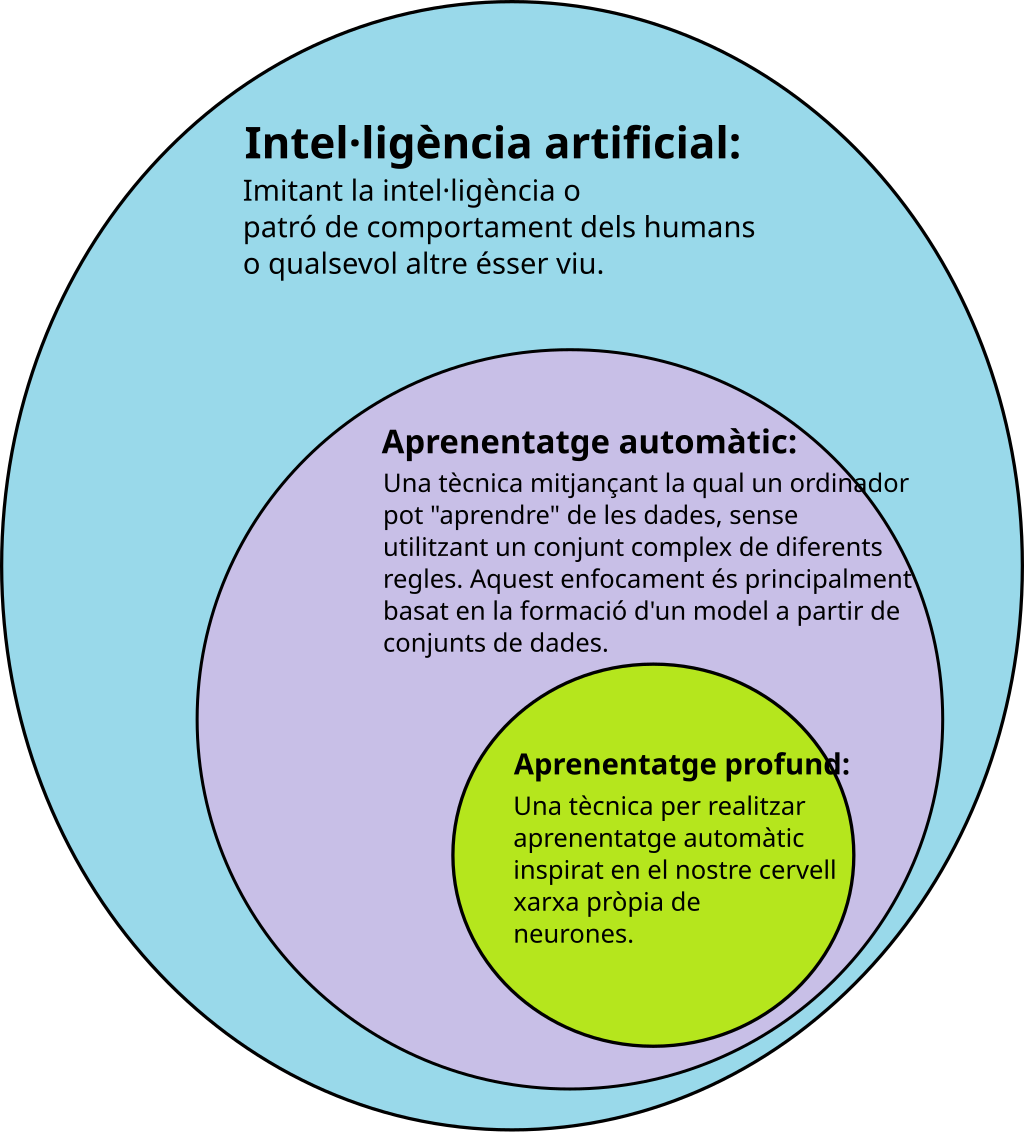
\includegraphics[width=0.2\textwidth]{./figures/Aprenentatge.png}
    \caption{Les capes que té l'IA per funcionar}
    \end{figure}
  \item \hypertarget{Software i Frameworks}{\textbf{Frameworks}}
      Segons INESDI~\cite{INESDI}:\\
      {\color{gray}``Un Frameworks és, en el camp de la informàtica, una estructura conceptual que proporciona un conjunt d'eines, biblioteques i patrons de disseny per facilitar el desenvolupament de programari.
      %En altres paraules, són marcs de treball que funcionen com un esquelet predefinit, i sobre els quals es pot construir una aplicació o programari.

     Pel que fa als seus components, inclouen biblioteques de codi reutilitzables, mòduls predefinits, regles d'arxiu i directori, patrons de disseny i convencions de codificació.''}\\

      %Un Framework, en diferencia, de la biblioteca per el control total que pot tenir el usuari en tema estructura, i organitzacio dels codis, en canvi, una biblioteca està en mans del desenvolupador i només tens accés en els codis que et convenin de la biblioteca. Malgrat la utilitat que propociona no satisfeix la IA de la actualitat i han hagut de desarollar uns Frameworks especifics per la IA, de tal manera en que facilita el desarollament i l'entrenament dels models de la IA.
      \begin{comment}
      \item[] \textbf{Software}
      El software és el conjunt de programes, instruccions i regles informàtiques que permeten executar tasques específiques en un ordinador o sistema.

      La relació entre el software i la IA funciona de la següent manera: d'una banda, el software dóna utilitat pràctica a la IA en àmbits reals, permetent codificar les seves tècniques i processar les grans quantitats de dades que necessita. D'altra banda, la IA aporta automatització a les tasques repetitives del software, estalviant temps i recursos. Aquesta interacció crea un benefici mutu que forma un cicle perfecte, on cadascú millora i potencia l'altre.
     \end{itemize}
      \end{comment}

   \item \hypertarget{Optimització i Ajustos}{\textbf{Mètodes d'Optimització en la Intel·ligència Artificial:Fonaments i Aplicacions}}\\
   \textbf{Introducció}\\
La intel·ligència artificial integra múltiples estratègies d'optimització, cadascuna adaptada als diferents models d'IA. A continuació, s'exploren els mètodes més destacats, amb una anàlisi dels mecanismes i les referències acadèmiques que hem utilitzat.

\begin{enumerate}
 \item \textbf{Retropropagació en Aprenentatge Profund:} La retropropagació (\textit{backpropagation}) és com el punt i coma en el text per les xarxes neuronals artificials. Aquest algorisme es basa en un procés iteratiu en dues fases:
    \begin{enumerate}
     \item \textbf{Fase de propagació endavant}: Les dades d'entrada es transmeten a través de les capes de la xarxa, generant una predicció. Durant aquest procés, cada neurona aplica una transformació lineal seguida d'una funció d'activació no lineal, com la \textit{\hyperlink{subsec:1}{funció unitat rectificada uniforme}} o la \textit{\hyperlink{3.7.1}{funció sigmoide}}.
%%%%%%Aquí a lo mejor hay un error de hyperlink, hay q verlo.
     \item \textbf{Fase de propagació enrere}: Es calcula l'error entre la predicció i el valor real utilitzant una funció de pèrdua (\textit{loss function}), com l'error quadràtic mitjà (\textit{Mean Squared Error}) per a problemes de regressió o l'entropia creuada (\textit{Cross-Entropy Loss}) per a classificació. Mitjançant la regla de la cadena (\textit{chain rule}), es determina la contribució de cada paràmetre a l'error global, obtenint els gradients $\partial L/\partial W$, on $L$ representa la pèrdua i $W$ els pesos de la xarxa.
%%%%%%No entiendo que explica el JiaJun
     \item \textbf{Actualització de paràmetres}: Els pesos s'ajusten en la direcció oposada al gradient, utilitzant variables del descens de gradient, com SGD \textit{\nameref{Algoritme_gradient}}, que aplica actualitzacions amb un subconjunt aleatori de dades, o optimitzadors més sofisticats com Adam (\textit{Adaptive Moment Estimation}), que adapta la taxa d'aprenentatge per a cada paràmetre.
    \end{enumerate}

 \textbf{Suport teòric}:
 \begin{quote}
 \textit{Rumelhart, D. E., Hinton, G. E., \& Williams, R. J. (1986). ``Learning representations by back-propagating errors.'' Nature, 323(6088), 533-536.}

 Aquest article seminal estableix els fonaments matemàtics de la retropropagació, demostrant la seva eficàcia per a l'entrenament de xarxes multicapa.
 \end{quote}
%%%%%%%%%%%%%%%%%%%%%%%%%%%%%%%%%%%%%%%%%%%%%%%%%%%%%Corrije JiaJun 240-367
 \item \textbf{Optimització en Models Generatius:} Els models generatius, com les xarxes generatives adversàries (GANs) i els autocidificadors variacionals (VAEs), empren tècniques d'optimització especialitzades.\\
